\documentclass[11pt, a4paper]{article}
\usepackage{graphicx}
\usepackage{amsmath}
\usepackage{listings}


\title{Assignment No 9} % Title

\author{Suhas C EE20B132} % Author name
\date{20-04-2022} % Date for the report


\begin{document}		
		
\maketitle % Insert the title, author and date
\section{Aim}
%Create new section;it is autonumbered
In this assignment, we continue our analysis of signals using Fourier Transforms. This time, we focus on finding transforms of non periodic functions. 
\section{Examples}
The worked examples in the assignment are given below:
Spectrum of $sin(\sqrt{2}t)$ is given below\newline
\begin{figure}[h!]
\centering
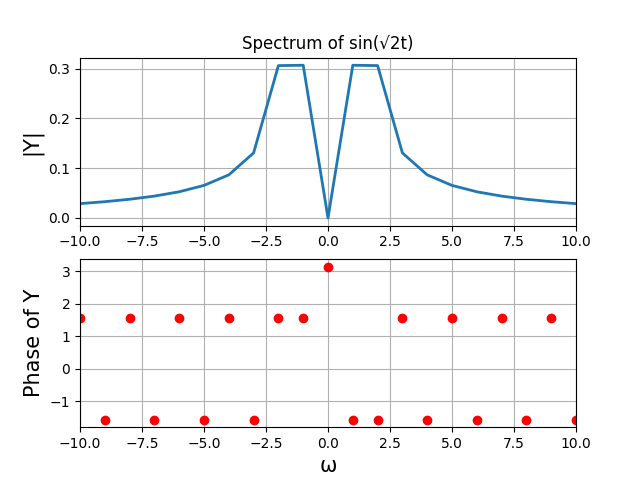
\includegraphics[scale=0.6]{fig10-1.png}
\caption{Spectrum of sin($\sqrt{2}t$)}
\label{fig:universe}
\end{figure}
\clearpage
Original function for which we want the DFT:
\begin{figure}[h!]
\centering
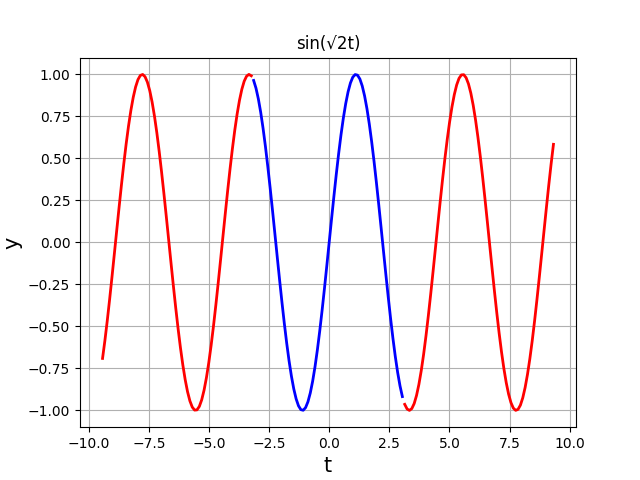
\includegraphics[scale=0.6]{fig10-2.png}
\caption{sin($\sqrt{2}t$)}
\label{fig:universe}
\end{figure}
As the DFT is computed over a finite time interval, we have actually plotted the DFT for this function
\begin{figure}[h!]
\centering
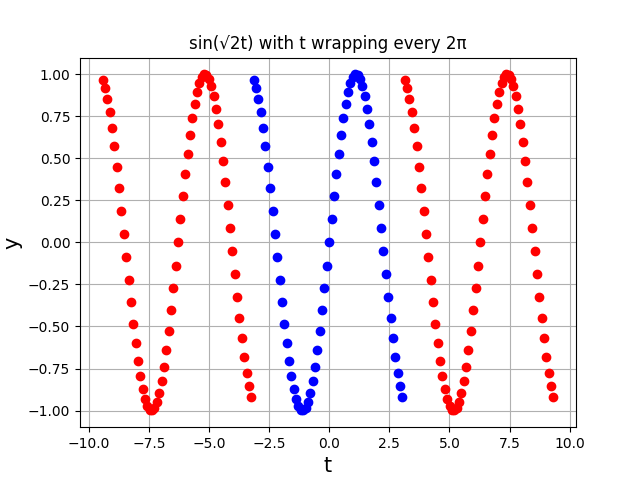
\includegraphics[scale=0.6]{fig10-3.png}
\caption{Spectrum of sin($\sqrt{2}t$)}
\label{fig:universe}
\end{figure}

These discontinuities lead to  non harmonic components in the FFT which decay as \(\frac{1}{\omega}\). To confirm
this, we plot the spectrum of the periodic ramp.
\begin{figure}[h!]
\centering
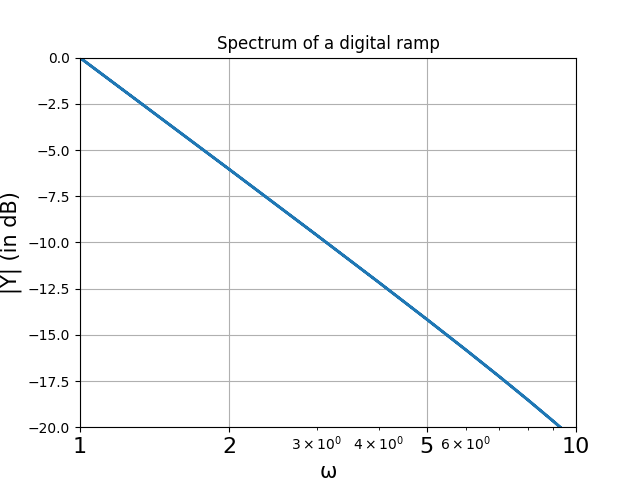
\includegraphics[scale=0.6]{fig10-4.png}
\caption{Spectrum of sin($\sqrt{2}t$)}
\label{fig:universe}
\end{figure}
\subsection{Windowing}
The hamming window removes discontinuities by attenuating the high frequency components that cause the discontinuities.
The hamming window function is given by
\begin{equation}
    x[n] = 0.54 + 0.46cos(\frac{2\pi n}{N-1})
\end{equation}

We multiply our signal with the hamming window and periodically extend it. The discontinuities nearly vanish.
\begin{figure}[h!]
\centering
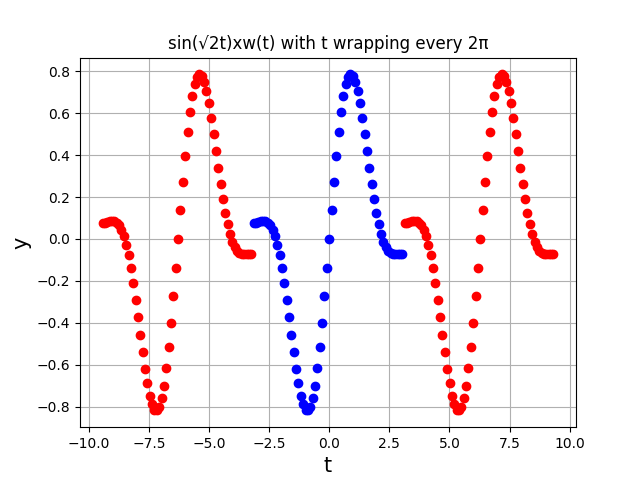
\includegraphics[scale=0.6]{fig10-5.png}
\caption{Spectrum of sin($\sqrt{2}t)*w(t)$}
\label{fig:universe}
\end{figure}
\clearpage
The spectrum that is obtained with a time period $2\pi$ is given below:
\begin{figure}[h!]
\centering
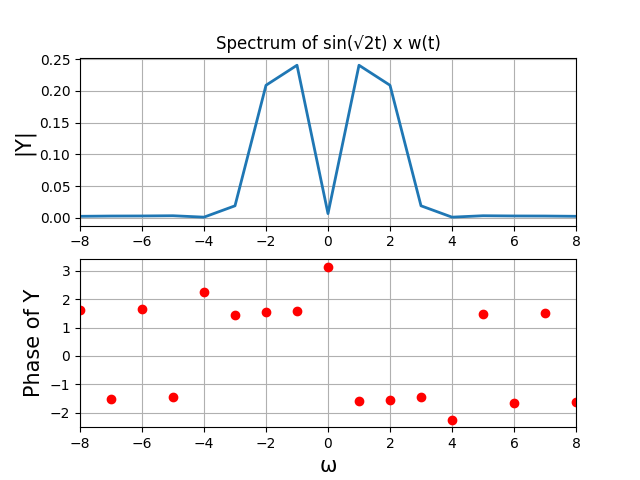
\includegraphics[scale=0.6]{fig10-6.png}
\caption{Spectrum of sin($\sqrt{2}t)*w(t)$}
\label{fig:universe}
\end{figure}

The spectrum that is obtained with a time period $8\pi$ has a sharper peak and is given below:
\begin{figure}[h!]
\centering
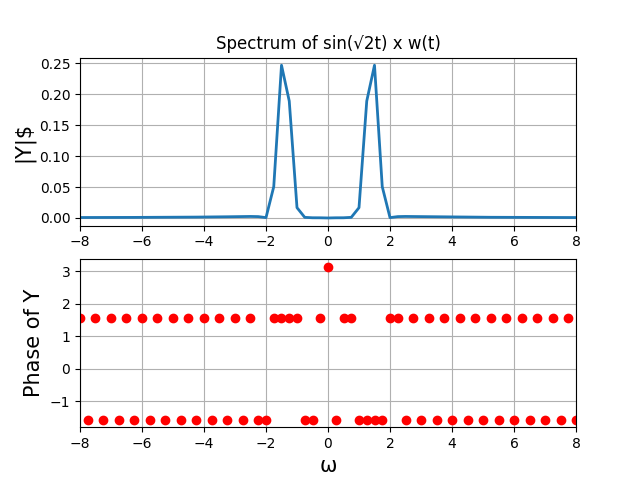
\includegraphics[scale=0.6]{fig10-7.png}
\caption{Spectrum of sin($\sqrt{2}t)*w(t)$}
\label{fig:universe}
\end{figure}
 
\section{Questions}
\subsection{Question 2}
In this question, we shall plot the FFT of $cos^3(0.86t)$
The FFT without the hamming Window:
\begin{figure}[h!]
\centering
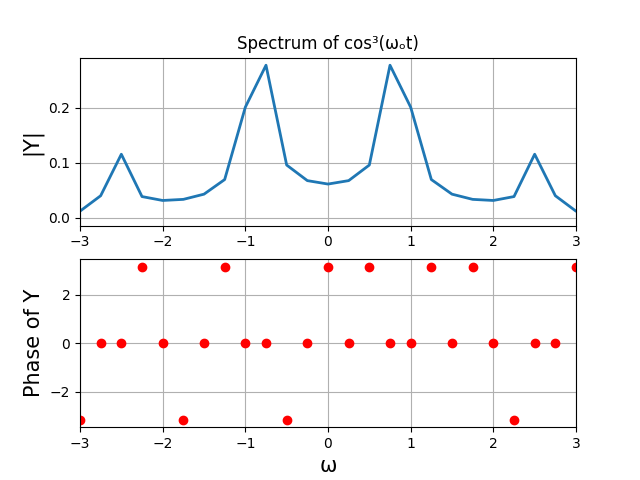
\includegraphics[scale=0.6]{10-8_NoWindow.png}
\label{fig:universe}
\end{figure}
\clearpage
We notice that a lot of the energy is stored in frequencies that aren't a part of the signal. After windowing, these frequencies are attenuated and hence the peaks are sharper in the windowed function. 

\subsection{Question 3}
We need to estimate $\omega$ and $\delta$ for a signal $\cos(\omega t + \delta)$ for 128 samples between $[-\pi,\pi)$. We estimate omega using a weighted average. We have to extract the digital spectrum of the signal and find the two peaks at $\pm\omega_0$, and estimate $\omega$ and $\delta$.
\begin{figure}[h!]
\centering
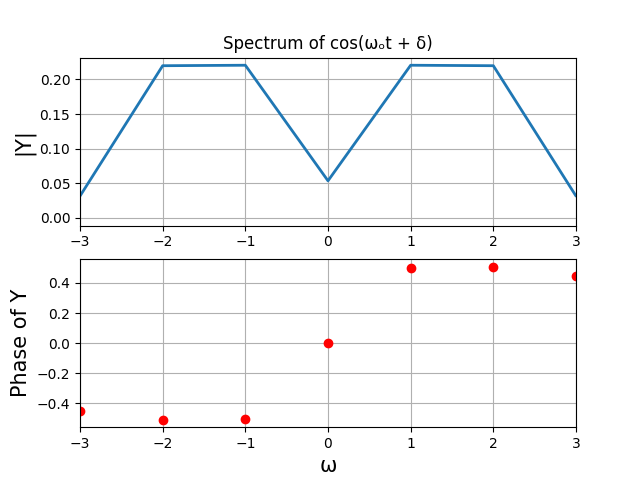
\includegraphics[scale=0.6]{10-8.png}
\caption{Fourier transform of $cos(1.5t+0.5)$}
\label{fig:universe}
\end{figure}

We estimate omega by performing a Mean average of $\omega$ over the magnitude of $|Y(j\omega)|$.
For delta we consider a widow on each half of $\omega$ (split into positive and negative values) and extract their mean slope. 

\newpage
\subsection{Question 4}
In this question we analyze a chirp signal which is an FM signal where frequency is directly proportional to time.
A chirp signal we shall consider is given by 
\begin{equation}
    f(t) = cos(16t(1.5 + \frac{t}{2\pi}))
\end{equation}
The FFT of the chirp is given by:
We note that the frequency response is spread between 5-50 rad/s. A large section of this range apears due to Gibbs phenomenon. On windowing, only frequencies between 16 and 32 rad/s remain.
\begin{figure}[h!]
\centering
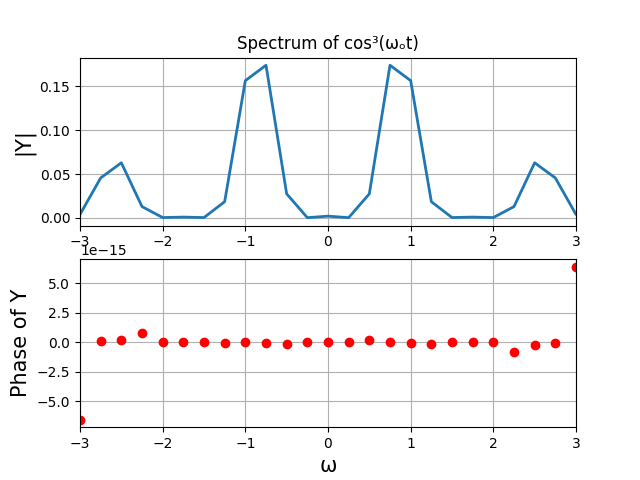
\includegraphics[scale=0.6]{10-8_Window.png}
\caption{Chirp function fourier transform, windowed}
\label{fig:universe}
\end{figure}

\section{Conclusion}
The DFT was obtained using a 2π periodic extension of the signal, and thus
the spectrum was found to be erroneous for a non periodic function. The
spectrum was rectified by the using a windowing technique, by employing the
Hamming window. Given a vector of cosine values in the a time interval, the
frequency and phase were estimated from the DFT spectrum, by using the
expectation value of the frequency and a parameter grid search for optimum
values. The DFT of a chirped signal was analysed and its time-frequency
plot showed the gradual variation of peak frequency of the spectrum with
time.


\end{document}
